% !TEX encoding = UTF-8
% !TEX TS-program = pdflatex
% !TEX root = ../tesi.tex

%**************************************************************
\chapter{Biztortion}
\label{cap:biztortion}
%**************************************************************

\intro{In questo capitolo viene descritta la realizzazione del processore di segnale audio digitale denominato \textit{Biztortion}, il quale implementa i diversi algoritmi di distorsione del segnale descritti nel capitolo precedente. Nel capitolo in questione verranno trattate in particolare l'analisi dei requisiti, la progettazione e la codifica del \gls{pluging} audio sopraccitato, in modo da coprire tutte le fasi del lavoro svolto e ottenere un prodotto software di qualità.}\\

%**************************************************************
\section{Analisi dei requisiti}
\label{sez:analisi-requisiti}
\subsection{Contesto di utilizzo}
Il software Biztortion, implementando diverse tipologie di algoritmi per la distorsione del segnale audio, viene sviluppato e distribuito come \gls{pluging} audio utilizzabile da qualsiasi utente all'interno della propria \gls{dawg} preferita. \\
Il processore di segnale in questione è pensato quindi per effettuare della \textbf{ricerca sonora} nel modo più creativo possibile, fornendo vari strumenti molto utili principalmente per la produzione di musica elettronica dance (e per questo è stata scelta un'elaborazione di \textbf{segnale audio stereofonico}), senza però escludere un possibile utilizzo più tecnico e legato alla post-produzione.

\subsection{Attori}
Il sistema ha come attore principale un \textbf{utente generico}, sul quale non vengono effettuate particolari supposizioni in quanto l'utente, una volta installato l'applicativo sul proprio computer e caricato sulla \gls{dawg} desiderata, ha la possibilità di accedere a tutte le funzionalità che offre il sistema stesso. Inoltre è utile sottolineare come il prodotto software, essendo \gls{opensourceg}, non necessita di effettuare particolari controlli e/o autenticazioni agli utenti che lo utilizzano.

\subsection{Casi d'uso}

Per lo studio dei casi di utilizzo del prodotto sono stati creati dei diagrammi di tipo \gls{umlg} per descrivere i casi d'uso\footcite{site:UseCase} (\textit{UC}) del software Biztortion. \\
I casi d'uso consistono in degli scenari di utilizzo del prodotto software e sono dedicati alla descrizione delle funzioni o servizi offerti da un sistema, così come sono percepiti e utilizzati dagli attori che interagiscono col sistema stesso. \\

\begin{figure}[h!] 
    \centering 
    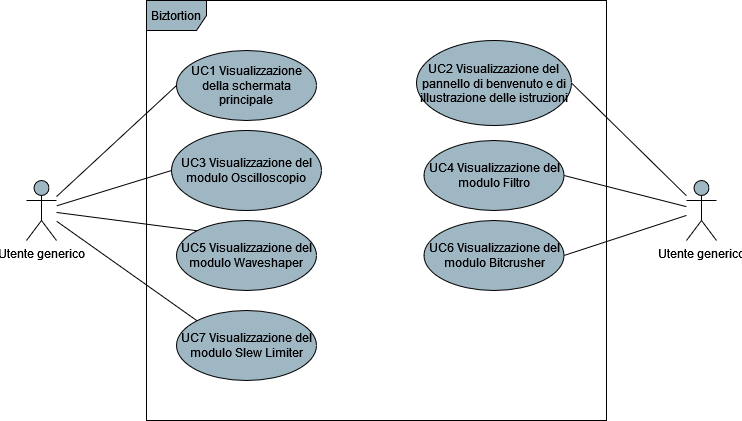
\includegraphics[width=0.9\columnwidth]{immagini/cap3/VisualizzazioneGenerale.png}
    \caption{Diagramma UML contenente i casi d'uso che riguardano la visualizzazione dei componenti dell'interfaccia}
\end{figure}

%\clearpage

% ----------------------------------- UC1 ----------------------------------------------

\begin{usecase}{1}{Visualizzazione della schermata principale}
\label{uc:1}
\usecaseactors{Utente generico}
\usecasepre{L'utente generico ha caricato con successo il \gls{pluging} nella propria \gls{dawg}}
\usecasedesc{L'utente generico visualizza i seguenti componenti nell'interfaccia principale del \gls{pluging}:
\begin{itemize}
    \item la \textit{Module Section}[\textbf{UC1.1}], ovvero una sezione dell'interfaccia riservata alla visualizzazione dei moduli per l'audio processing o al pannello di benvenuto[\textbf{UC2}];
    \item la \textit{Chain Section}[\textbf{UC1.2}], ovvero una sezione dell'interfaccia riservata alla visualizzazione della catena di \textit{ChainPosition}, i quali possono rappresentare un modulo già istanziato [\textbf{UC1.2.1}] o non ancora instanziato [\textbf{UC1.2.2}];
    \item la \textit{Input Section}[\textbf{UC1.3}], ovvero una sezione dell'interfaccia riservata al controllo del guadagno e il monitoraggio del segnale in input;
    \item la \textit{Output Section}[\textbf{UC1.4}], ovvero una sezione dell'interfaccia riservata al controllo del guadagno e il monitoraggio del segnale in output;
    \item il nome del \gls{pluging} come titolo sulla parte superiore dell'interfaccia;
    \item un link che indirizza l'utente al profilo Github di Gabriel Bizzo per visualizzare il codice sorgente del software e varie informazioni extra sul progetto;
    \item un pulsante che genera un pannello di benvenuto all'utente[\textbf{UC2}], contenente inoltre le istruzioni basilari per l'utilizzo del \gls{pluging}, sulla \textit{Module Section}.
\end{itemize}
}
\usecasepost{L'utente generico visualizza la schermata principale del software}
\end{usecase}

\begin{figure}[h!] 
    \centering 
    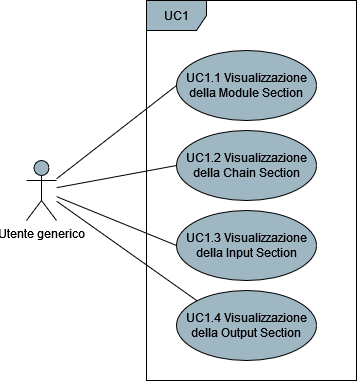
\includegraphics[width=0.6\columnwidth]{immagini/cap3/UC1.png}
    \caption{Use Case - UC1: Visualizzazione della schermata principale}
\end{figure}

% ----------------------------------- UC1.1 ----------------------------------------------

\begin{usecase}{1.1}{Visualizzazione della Module Section}
\usecaseactors{Utente generico}
\usecasepre{L'utente generico sta visualizzando la schermata principale del software}
\usecasedesc{L'utente generico nella schermata denominata \textit{Module Section} visualizza due possibili contenuti:
\begin{itemize}
    \item un \textit{modulo per il processing del segnale audio} [\textbf{UC3-7}];
    \item un \textit{pannello di benvenuto} all'utente [\textbf{UC2}].
\end{itemize}
}
\usecasepost{L'utente generico visualizza il contenuto della Module Section}
\end{usecase}

% ----------------------------------- UC1.2 ----------------------------------------------

\begin{usecase}{1.2}{Visualizzazione della Chain Section}
\usecaseactors{Utente generico}
\usecasepre{L'utente generico sta visualizzando la schermata principale del software}
\usecasedesc{L'utente generico nella schermata denominata \textit{Chain Section} visualizza un insieme di otto Chain Position, posizionati in ordine uno di fianco all'altro. Questi elementi contenuti in questa sezione possono essere di due tipologie:
\begin{itemize}
    \item una Chain Position che rappresenta un modulo \textit{istanziato} e presente nella catena di elaborazione dell'audio [\textbf{UC1.2.1}];
    \item una Chain Position che rappresenta un modulo \textit{NON istanziato}, e quindi non effettua alcuna operazione sul segnale audio [\textbf{UC1.2.2}].
\end{itemize}
}
\usecasepost{L'utente generico visualizza il contenuto della Chain Section}
\end{usecase}

\begin{figure}[h!] 
    \centering 
    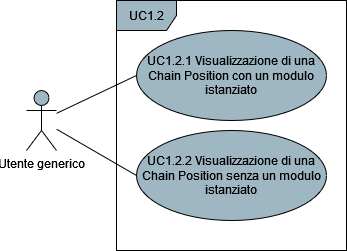
\includegraphics[width=0.6\columnwidth]{immagini/cap3/UC1_2.png}
    \caption{Use Case - UC1.2: Visualizzazione della Chain Section}
\end{figure}

% ----------------------------------- UC1.2.1 ----------------------------------------------

\begin{usecase}{1.2.1}{Visualizzazione di una Chain Position con un modulo istanziato}
\usecaseactors{Utente generico}
\usecasepre{L'utente generico sta visualizzando una Chain Position che rappresenta un modulo attualmente istanziato nella catena di elaborazione del segnale}
\usecasedesc{L'utente generico visualizza i seguenti componenti contenuti nella sezione in questione:
\begin{itemize}
    \item il numero di posizione nella catena di elaborazione del segnale;
    \item il pulsante per l'eliminazione del modulo attualmente istanziato dalla catena di elaborazione dell'audio [\textbf{UC11}];
    \item il pulsante per l'accesso al modulo attualmente istanziato [\textbf{UC12}].
\end{itemize}
}
\usecasepost{L'utente generico visualizza il contenuto della Chain Position rappresentante un modulo attualmente istanziato nella catena di elaborazione del segnale}
\end{usecase}

% ----------------------------------- UC1.2.2 ----------------------------------------------

\begin{usecase}{1.2.2}{Visualizzazione di una Chain Position senza un modulo istanziato}
\usecaseactors{Utente generico}
\usecasepre{L'utente generico sta visualizzando una Chain Position che non rappresenta nessun modulo istanziato nella catena di elaborazione del segnale}
\usecasedesc{L'utente generico visualizza i seguenti componenti contenuti nella sezione in questione:
\begin{itemize}
    \item il numero di posizione nella catena di elaborazione del segnale;
    \item il pulsante per l'istanziazione di un nuovo modulo nella catena di elaborazione dell'audio alla posizione indicata dal numero del punto precedente [\textbf{UC10}].
\end{itemize}
}
\usecasepost{L'utente generico visualizza il contenuto della Chain Position non rappresentante alcun modulo, corrispondente dunque ad una posizione libera nella catena di elaborazione dell'audio}
\end{usecase}

% ----------------------------------- UC1.3 ----------------------------------------------

\begin{usecase}{1.3}{Visualizzazione della Input Section}
\usecaseactors{Utente generico}
\usecasepre{L'utente generico sta visualizzando la schermata principale del software}
\usecasedesc{L'utente generico nella schermata denominata \textit{Input Section} visualizza i seguenti componenti:
\begin{itemize}
    \item il titolo della sezione in questione;
    \item un misuratore di livello del segnale in ingresso al software;
    \item un potenziometro per la modifica del guadagno del segnale in ingresso al software.
\end{itemize}
}
\usecasepost{L'utente generico visualizza i componenti costitutivi della Input Section}
\end{usecase}

% ----------------------------------- UC1.4 ----------------------------------------------

\begin{usecase}{1.4}{Visualizzazione della Output Section}
\usecaseactors{Utente generico}
\usecasepre{L'utente generico sta visualizzando la schermata principale del software}
\usecasedesc{L'utente generico nella schermata denominata \textit{Output Section} visualizza i seguenti componenti:
\begin{itemize}
    \item il titolo della sezione in questione;
    \item un misuratore di livello del segnale in uscita al software;
    \item un potenziometro per la modifica del guadagno del segnale in uscita al software.
\end{itemize}
}
\usecasepost{L'utente generico visualizza i componenti costitutivi della Output Section}
\end{usecase}

% ----------------------------------- UC2 ----------------------------------------------

\begin{usecase}{2}{Visualizzazione del pannello di benvenuto e di illustrazione delle istruzioni}
\usecaseactors{Utente generico}
\usecasepre{L'utente generico visualizza la schermata principale del software e si verifica una delle seguenti condizioni:
\begin{itemize}
    \item l'utente effettua l'istanziazione del software nella propria \gls{dawg};
    \item l'utente elimina un modulo dalla catena di elaborazione del segnale [\textbf{UC11}];
    \item non sono presenti moduli istanziati nella catena di elaborazione del segnale;
    \item l'utente clicca sul pulsante, visualizzabile nella schermata principale [\textbf{UC1}], per visualizzare le istruzioni del \gls{pluging} in questione.
\end{itemize}
}
\usecasedesc{L'utente generico visualizza i seguenti componenti nella \textit{Module Section}:
\begin{itemize}
    \item il nome e il logo del software;
    \item un messaggio di benvenuto;
    \item un breve elenco di istruzioni utili all'utente per capire il funzionamento del \gls{pluging} audio.
\end{itemize}
}
\usecasepost{L'utente generico visualizza una sezione contenente un messaggio di benvenuto ed un elenco di istruzioni utili per il corretto utilizzo del software}
\label{uc:2}
\end{usecase}

% ----------------------------------- UC3 ----------------------------------------------

\begin{usecase}{3}{Visualizzazione del modulo Oscilloscopio}
\usecaseactors{Utente generico}
\usecasepre{L'utente generico visualizza la schermata principale del software e si verifica una delle seguenti condizioni:
\begin{itemize}
    \item l'utente effettua l'istanziazione del modulo Oscilloscopio in una specifica Chain Position [\textbf{UC10}];
    \item l'utente accede al modulo Oscilloscopio, attualmente istanziato in una specifica Chain Position, attraverso l'apposito pulsante [\textbf{UC12}].
\end{itemize}}
\usecasedesc{L'utente generico visualizza i seguenti componenti, corrispondenti al contenuto del modulo Oscilloscopio, nella \textit{Module Section}:
    \begin{itemize}
        \item il titolo del modulo;
        \item un \textit{oscilloscopio} per visualizzare la forma d'onda del segnale in ingresso;
        \item i parametri utilizzabili dall'utente per la modifica della visualizzazione del segnale audio[\textbf{UC14-15}], e in particolare:
            \begin{itemize}
                \item il pulsante \textit{bypass};
                \item un pulsante \textit{freeze};
                \item un potenziometro \textit{zoom verticale};
                \item un potenziometro \textit{zoom orizzontale}.
            \end{itemize}
    \end{itemize}
}
\usecasepost{L'utente generico visualizza tutte le informazioni, parametri e componenti grafici necessari al corretto utilizzo del modulo Oscilloscopio}
\end{usecase}

% ----------------------------------- UC4 ----------------------------------------------

\begin{usecase}{4}{Visualizzazione del modulo Filtro}
\usecaseactors{Utente generico}
\usecasepre{L'utente generico visualizza la schermata principale del software e si verifica una delle seguenti condizioni:
\begin{itemize}
    \item l'utente effettua l'istanziazione del modulo Filtro in una specifica Chain Position [\textbf{UC10}];
    \item l'utente accede al modulo Filtro, attualmente istanziato in una specifica Chain Position, attraverso l'apposito pulsante [\textbf{UC12}].
\end{itemize}}
\usecasedesc{L'utente generico visualizza i seguenti componenti, corrispondenti al contenuto del modulo Filtro, nella \textit{Module Section}:
    \begin{itemize}
        \item il titolo del modulo;
        \item un \textit{analizzatore di spettro} per visualizzare lo spettro frequenziale del segnale;
        \item un pulsante \textit{spectrum analyzer};
        \item un componente grafico per visualizzare la \textit{curva di risposta del filtro}, la quale comprende i filtri Passa Basso, Passa Banda e Passa Alto;
        \item i parametri utilizzabili dall'utente per la modifica del segnale audio[\textbf{UC16}], e in particolare:
            \begin{itemize}
                \item il pulsante \textit{bypass};
                \item un potenziometro \textit{Low Pass frequency};
                \item un potenziometro \textit{Low Pass order};
                \item un potenziometro \textit{Peak frequency};
                \item un potenziometro \textit{Peak gain};
                \item un potenziometro \textit{Peak quality};
                \item un potenziometro \textit{High Pass frequency};
                \item un potenziometro \textit{High Pass order}.
            \end{itemize}
    \end{itemize}
}
\usecasepost{L'utente generico visualizza tutte le informazioni, parametri e componenti grafici necessari al corretto utilizzo del modulo Filtro}
\end{usecase}

% ----------------------------------- UC5 ----------------------------------------------

\begin{usecase}{5}{Visualizzazione del modulo Waveshaper}
\usecaseactors{Utente generico}
\usecasepre{L'utente generico visualizza la schermata principale del software e si verifica una delle seguenti condizioni:
\begin{itemize}
    \item l'utente effettua l'istanziazione del modulo Waveshaper in una specifica Chain Position [\textbf{UC10}];
    \item l'utente accede al modulo Waveshaper, attualmente istanziato in una specifica Chain Position, attraverso l'apposito pulsante [\textbf{UC12}].
\end{itemize}}
\usecasedesc{L'utente generico visualizza i seguenti componenti, corrispondenti al contenuto del modulo Waveshaper, nella \textit{Module Section}:
    \begin{itemize}
        \item il titolo del modulo;
        \item un grafico che rappresenta la \textit{funzione di trasferimento} applicata al segnale in ingresso;
        \item i parametri utilizzabili dall'utente per la modifica del segnale audio[\textbf{UC17}], e in particolare:
            \begin{itemize}
                \item il pulsante \textit{bypass};
                \item un potenziometro \textit{drive};
                \item un potenziometro \textit{mix};
                \item un potenziometro \textit{symmetry};
                \item un potenziometro \textit{bias};
                \item un potenziometro \textit{tanh amplitude};
                \item un potenziometro \textit{tanh slope};
                \item un potenziometro \textit{sine amplitude};
                \item un potenziometro \textit{sine frequency}.
            \end{itemize}
    \end{itemize}
}
\usecasepost{L'utente generico visualizza tutte le informazioni, parametri e componenti grafici necessari al corretto utilizzo del modulo Waveshaper}
\end{usecase}

% ----------------------------------- UC6 ----------------------------------------------

\begin{usecase}{6}{Visualizzazione del modulo Bitcrusher}
\usecaseactors{Utente generico}
\usecasepre{L'utente generico visualizza la schermata principale del software e si verifica una delle seguenti condizioni:
\begin{itemize}
    \item l'utente effettua l'istanziazione del modulo Bitcrusher in una specifica Chain Position [\textbf{UC10}];
    \item l'utente accede al modulo Bitcrusher, attualmente istanziato in una specifica Chain Position, attraverso l'apposito pulsante [\textbf{UC12}].
\end{itemize}}
\usecasedesc{L'utente generico visualizza i seguenti componenti, corrispondenti al contenuto del modulo Bitcrusher, nella \textit{Module Section}:
    \begin{itemize}
        \item il titolo del modulo;
        \item i parametri utilizzabili dall'utente per la modifica del segnale audio [\textbf{UC18}], e in particolare:
            \begin{itemize}
                \item il pulsante \textit{bypass};
                \item un potenziometro \textit{drive};
                \item un potenziometro \textit{mix};
                \item un potenziometro \textit{symmetry};
                \item un potenziometro \textit{bias};
                \item un potenziometro \textit{rate reduction};
                \item un potenziometro \textit{bit reduction};
                \item un potenziometro \textit{dithering}.
            \end{itemize}
    \end{itemize}
}
\usecasepost{L'utente generico visualizza tutte le informazioni, parametri e componenti grafici necessari al corretto utilizzo del modulo Bitcrusher}
\end{usecase}

% ----------------------------------- UC7 ----------------------------------------------

\begin{usecase}{7}{Visualizzazione del modulo Slew Limiter}
\usecaseactors{Utente generico}
\usecasepre{L'utente generico visualizza la schermata principale del software e si verifica una delle seguenti condizioni:
\begin{itemize}
    \item l'utente effettua l'istanziazione del modulo Slew Limiter in una specifica Chain Position [\textbf{UC10}];
    \item l'utente accede al modulo Slew Limiter, attualmente istanziato in una specifica Chain Position, attraverso l'apposito pulsante [\textbf{UC12}].
\end{itemize}}
\usecasedesc{L'utente generico visualizza i seguenti componenti, corrispondenti al contenuto del modulo Slew Limiter, nella \textit{Module Section}:
    \begin{itemize}
        \item il titolo del modulo;
        \item i parametri utilizzabili dall'utente per la modifica del segnale audio [\textbf{UC19}], e in particolare:
            \begin{itemize}
                \item il pulsante \textit{bypass};
                \item un potenziometro \textit{drive};
                \item un potenziometro \textit{mix};
                \item un potenziometro \textit{symmetry};
                \item un potenziometro \textit{bias};
                \item un potenziometro \textit{rise};
                \item un potenziometro \textit{fall};
                \item un pulsante a doppio stato \textit{DC filter}.
            \end{itemize}
    \end{itemize}
}
\usecasepost{L'utente generico visualizza tutte le informazioni, parametri e componenti grafici necessari al corretto utilizzo del modulo Slew Limiter}
\end{usecase}

% -----------------------------------------------------------------------------
\clearpage

\begin{figure}[h!] 
    \centering 
    \includegraphics[width=0.9\columnwidth]{immagini/cap3/FunzionalitàGenerale.png}
    \caption{Diagramma UML contenente i casi d'uso che riguardano le funzionalità offerte dai  moduli istanziabili nel sistema}
\end{figure}

% ----------------------------------- UC8 ----------------------------------------------

\begin{usecase}{8}{Reset del valore di picco e del segnale di clip}
\usecaseactors{Utente generico}
\usecasepre{L'utente generico sta visualizzando la \textit{Input Section} o la \textit{Output Section}}
\usecasedesc{L'utente generico, visualizzando il misuratore di livello, ha la possibilità di resettare il massimo valore di picco rilevato, andando inoltre a disabilitare il segnale di clip (rosso nel caso in cui il segnale supera i 0 \gls{dbfsg}).}
\usecasepost{L'utente generico effettua il reset del valore di picco e del segnale di clip nel misuratore di livello presente nella \textit{Input Section} o nella \textit{Output Section}}
\end{usecase}

% ----------------------------------- UC9 ----------------------------------------------

\begin{usecase}{9}{Modifica del guadagno del segnale}
\usecaseactors{Utente generico}
\usecasepre{L'utente generico sta visualizzando la \textit{Input Section} o la \textit{Output Section}}
\usecasedesc{L'utente generico, visualizzando il potenziometro relativo al guadagno del segnale, ha la possibilità di modificare il guadagno del segnale in ingresso nella sezione in questione.}
\usecasepost{L'utente generico effettua la modifica del guadagno del segnale in ingresso nella \textit{Input Section} o nella \textit{Output Section}}
\end{usecase}

% ----------------------------------- UC10 ----------------------------------------------

\begin{usecase}{10}{Aggiunta di un nuovo modulo}
\usecaseactors{Utente generico}
\usecasepre{L'utente generico visualizza la \textit{Chain Section}[\textbf{UC1.2}] ed ha selezionato una Chain Position senza un modulo istanziato[\textbf{UC1.2.2}]}
\usecasedesc{L'utente generico, con l'obiettivo di istanziare un nuovo modulo nella \textit{Chain Position} desiderata, deve eseguire le seguenti operazioni:
    \begin{enumerate}
        \item cliccare sul pulsante, presente nella \textit{Chain Position} in questione, per istanziare un nuovo modulo nella catena di elaborazione del segnale;
        \item selezionare il modulo desiderato dal menù a tendina comparso nella \textit{Module Section}.
    \end{enumerate}
    Dopo aver completato la procedura appena descritta il modulo risulterà istanziato nella catena di elaborazione del segnale nella posizione descritta dal numero della \textit{Chain Position} in questione e il modulo risulterà visibile ed interagibile nella \textit{Module Section}.
}
\usecasepost{L'utente generico istanzia un nuovo modulo nella catena di elaborazione del segnale, il quale diventa visibile ed interagibile attraverso l'interfaccia grafica del software}
\end{usecase}

% ----------------------------------- UC11 ----------------------------------------------

\begin{usecase}{11}{Rimozione di un modulo istanziato}
\usecaseactors{Utente generico}
\usecasepre{L'utente generico visualizza la \textit{Chain Section}[\textbf{UC1.2}] ed ha selezionato una Chain Position con un modulo attualmente istanziato[\textbf{UC1.2.1}]}
\usecasedesc{L'utente generico, con l'obiettivo di eliminare il modulo attualmente istanziato nella \textit{Chain Position} desiderata, deve eseguire le seguenti operazioni:
    \begin{enumerate}
        \item \item cliccare sul pulsante, presente nella \textit{Chain Position} in questione, per eliminare il modulo attualmente istanziato dalla catena di elaborazione del segnale.
    \end{enumerate}
    Dopo aver completato la procedura appena descritta il modulo risulterà rimosso dalla catena di elaborazione del segnale e dalla \textit{Module Section}.
}
\usecasepost{L'utente generico rimuove un modulo precedentemente istanziato nella catena di elaborazione del segnale}
\end{usecase}

% ----------------------------------- UC12 ----------------------------------------------

\begin{usecase}{12}{Accesso ad un modulo istanziato}
\usecaseactors{Utente generico}
\usecasepre{L'utente generico visualizza la \textit{Chain Section}[\textbf{UC1.2}] ed ha selezionato una Chain Position con un modulo attualmente istanziato[\textbf{UC1.2.1}]}
\usecasedesc{L'utente generico, con l'obiettivo di accedere all'interfaccia grafica per interagire con il modulo attualmente istanziato nella \textit{Chain Position} desiderata, deve eseguire le seguenti operazioni:
    \begin{enumerate}
        \item \item cliccare sul pulsante, presente nella \textit{Chain Position} in questione, per accedere al modulo istanziato dalla catena di elaborazione del segnale.
    \end{enumerate}
    Dopo aver completato la procedura appena descritta il modulo risulterà visibile ed interagibile nella \textit{Module Section}.
}
\usecasepost{L'utente generico accede ad un modulo istanziato nella catena di elaborazione del segnale}
\end{usecase}

% ----------------------------------- UC13 ----------------------------------------------

\begin{usecase}{13}{Scatto di un'istantanea nel modulo Oscilloscopio}
\usecaseactors{Utente generico}
\usecasepre{L'utente generico visualizza il modulo Oscilloscopio [\textbf{UC3}], il quale risulta istanziato in una determinata \textit{Chain Position} e quindi presente nella catena di elaborazione del segnale}
\usecasedesc{L'utente generico ha la possibilità di effettuare un'istantanea sul componente grafico corrispondente all'oscilloscopio cliccando sull'apposito pulsante \textit{freeze}.
}
\usecasepost{L'utente generico effettua un'istantanea sul componente grafico corrispondente all'oscilloscopio}
\end{usecase}

% ----------------------------------- UC14 ----------------------------------------------

\begin{usecase}{14}{Modifica dei parametri nel modulo Oscilloscopio}
\usecaseactors{Utente generico}
\usecasepre{L'utente generico visualizza il modulo Oscilloscopio[\textbf{UC3}], il quale risulta istanziato in una determinata \textit{Chain Position} e quindi presente nella catena di elaborazione del segnale}
\usecasedesc{L'utente generico ha la possibilità influenzare l'azione del modulo sulla catena di elaborazione interagendo con i suoi parametri. In particolare le modifiche effettuabili dall'utente sono le seguenti:
\begin{itemize}
    \item il pulsante \textit{bypass} permette di controllare l'attivazione del modulo sulla catena di elaborazione del segnale;
    \item il potenziometro \textit{zoom verticale} permette l'aggiustamento della visualizzazione verticale della forma d'onda;
    \item \textit{zoom orizzontale} permette l'aggiustamento della visualizzazione orizzontale della forma d'onda.
\end{itemize}
}
\usecasepost{L'utente generico, interagendo con i parametri del modulo Oscilloscopio, modifica il segnale nella modalità descritta precedentemente}
\end{usecase}

% ----------------------------------- UC15 ----------------------------------------------

\begin{usecase}{15}{Attivazione dell'analizzatore spettrale nel modulo Filtro}
\usecaseactors{Utente generico}
\usecasepre{L'utente generico visualizza il modulo Filtro [\textbf{UC4}], il quale risulta istanziato in una determinata \textit{Chain Position} e quindi presente nella catena di elaborazione del segnale}
\usecasedesc{L'utente generico ha la possibilità di attivare l'analizzatore dello spettro frequenziale del segnale cliccando sull'apposito pulsante \textit{spectrum analyzer}.
}
\usecasepost{L'utente generico attiva l'analizzatore dello spettro frequenziale}
\end{usecase}

% ----------------------------------- UC16 ----------------------------------------------

\begin{usecase}{16}{Modifica dei parametri nel modulo Filtro}
\usecaseactors{Utente generico}
\usecasepre{L'utente generico visualizza il modulo Filtro[\textbf{UC4}], il quale risulta istanziato in una determinata \textit{Chain Position} e quindi presente nella catena di elaborazione del segnale}
\usecasedesc{L'utente generico ha la possibilità influenzare l'azione del modulo sulla catena di elaborazione interagendo con i suoi parametri. In particolare le modifiche effettuabili dall'utente sono le seguenti:
\begin{itemize}
    \item il pulsante \textit{bypass} permette di controllare l'attivazione del modulo sulla catena di elaborazione del segnale;
    \item il potenziometro \textit{Low Pass frequency} permette l'aggiustamento della frequenza del filtro \gls{iirg} Passa Basso;
    \item il potenziometro \textit{Low Pass order} permette l'aggiustamento dell'ordine del filtro \gls{iirg} Passa Basso;
    \item il potenziometro \textit{Peak frequency} permette l'aggiustamento della frequenza del filtro \gls{iirg} Passa Banda;
    \item il potenziometro \textit{Peak gain} permette l'aggiustamento del guadagno del filtro \gls{iirg} Passa Banda;
    \item il potenziometro \textit{Peak quality} permette l'aggiustamento della qualità del filtro \gls{iirg} Passa Banda;
    \item il potenziometro \textit{High Pass frequency} permette l'aggiustamento della frequenza del filtro \gls{iirg} Passa Alto;
    \item il potenziometro \textit{High Pass order} permette l'aggiustamento dell'ordine del filtro \gls{iirg} Passa Alto.
\end{itemize}
}
\usecasepost{L'utente generico, interagendo con i parametri del modulo Filtro, modifica il segnale nella modalità descritta precedentemente}
\end{usecase}

% ----------------------------------- UC17 ----------------------------------------------

\begin{usecase}{17}{Modifica dei parametri nel modulo Waveshaper}
\usecaseactors{Utente generico}
\usecasepre{L'utente generico visualizza il modulo Waveshaper[\textbf{UC5}], il quale risulta istanziato in una determinata \textit{Chain Position} e quindi presente nella catena di elaborazione del segnale}
\usecasedesc{L'utente generico ha la possibilità influenzare l'azione del modulo sulla catena di elaborazione interagendo con i suoi parametri. In particolare le modifiche effettuabili dall'utente sono le seguenti:
\begin{itemize}
    \item il pulsante \textit{bypass} permette di controllare l'attivazione del modulo sulla catena di elaborazione del segnale;
    \item il potenziometro \textit{drive} permette di gestire il guadagno del segnale in ingresso;
    \item il potenziometro \textit{mix} permette il dosaggio tra il segnale originale e quello modificato;
    \item il potenziometro \textit{symmetry} permette il dosaggio dell' effetto dato dalla distorsione nelle due diverse zone dell'onda sonora, ovvero nella fase positiva e negativa;
    \item il potenziometro \textit{bias} permette di determinare la separazione tra la zona positiva e quella negativa dell'onda sonora in punti diversi rispetto all'origine;
    \item il potenziometro \textit{tanh amplitude} permette di determinare l'ampiezza della funzione arcotangente utilizzata nella funzione di trasferimento;
    \item il potenziometro \textit{tanh slope} permette di determinare l'inclinazione della funzione arcotangente utilizzata nella funzione di trasferimento;
    \item il potenziometro \textit{sine amplitude} permette di determinare l'ampiezza della funzione sinusoidale utilizzata nella funzione di trasferimento;
    \item il potenziometro \textit{sine frequency} permette di determinare la frequenza della funzione sinusoidale utilizzata nella funzione di trasferimento.
\end{itemize}
}
\usecasepost{L'utente generico, interagendo con i parametri del modulo Waveshaper, modifica il segnale nella modalità descritta precedentemente}
\end{usecase}

% ----------------------------------- UC18 ----------------------------------------------

\begin{usecase}{18}{Modifica dei parametri nel modulo Bitcrusher}
\usecaseactors{Utente generico}
\usecasepre{L'utente generico visualizza il modulo Bitcrusher[\textbf{UC6}], il quale risulta istanziato in una determinata \textit{Chain Position} e quindi presente nella catena di elaborazione del segnale}
\usecasedesc{L'utente generico ha la possibilità influenzare l'azione del modulo sulla catena di elaborazione interagendo con i suoi parametri. In particolare le modifiche effettuabili dall'utente sono le seguenti:
\begin{itemize}
    \item il pulsante \textit{bypass} permette di controllare l'attivazione del modulo sulla catena di elaborazione del segnale;
    \item il potenziometro \textit{drive} permette di gestire il guadagno del segnale in ingresso;
    \item il potenziometro \textit{mix} permette il dosaggio tra il segnale originale e quello modificato;
    \item il potenziometro \textit{symmetry} permette il dosaggio dell' effetto dato dalla distorsione nelle due diverse zone dell'onda sonora, ovvero nella fase positiva e negativa;
    \item il potenziometro \textit{bias} permette di determinare la separazione tra la zona positiva e quella negativa dell'onda sonora in punti diversi rispetto all'origine;
    \item il potenziometro \textit{rate reduction} permette di determinare la riduzione della frequenza di campionamento utilizzata per la degradazione del campionamento del segnale;
    \item il potenziometro \textit{bit reduction} permette di determinare la riduzione della profondità di bit utilizzata per la degradazione della quantizzazione del segnale;
    \item il potenziometro \textit{dithering} permette di determinare la percentuale di rumore bianco da introdurre nel segnale per distorcere ulteriormente il segnale oppure per effettuare del \gls{ditheringg}, ammorbidendo quindi gli artefatti introdotti con la degradazione del segnale.
\end{itemize}
}
\usecasepost{L'utente generico, interagendo con i parametri del modulo Bitcrusher, modifica il segnale nella modalità descritta precedentemente}
\end{usecase}

% ----------------------------------- UC19 ----------------------------------------------

\begin{usecase}{19}{Modifica dei parametri nel modulo Slew Limiter}
\usecaseactors{Utente generico}
\usecasepre{L'utente generico visualizza il modulo Slew Limiter[\textbf{UC7}], il quale risulta istanziato in una determinata \textit{Chain Position} e quindi presente nella catena di elaborazione del segnale}
\usecasedesc{L'utente generico ha la possibilità influenzare l'azione del modulo sulla catena di elaborazione interagendo con i suoi parametri. In particolare le modifiche effettuabili dall'utente sono le seguenti:
\begin{itemize}
    \item il pulsante \textit{bypass} permette di controllare l'attivazione del modulo sulla catena di elaborazione del segnale;
    \item il potenziometro \textit{drive} permette di gestire il guadagno del segnale in ingresso;
    \item il potenziometro \textit{mix} permette il dosaggio tra il segnale originale e quello modificato;
    \item il potenziometro \textit{symmetry} permette il dosaggio dell' effetto dato dalla distorsione nelle due diverse zone dell'onda sonora, ovvero nella fase positiva e negativa;
    \item il potenziometro \textit{bias} permette di determinare la separazione tra la zona positiva e quella negativa dell'onda sonora in punti diversi rispetto all'origine;
    \item il potenziometro \textit{rise} permette di scegliere la soglia di velocità massima sopra alla quale essa stessa viene limitata nel tempo sul segnale in uscita durante la fase di salita dell'onda sonora;
    \item il potenziometro \textit{fall} permette di scegliere la soglia di velocità massima sopra alla quale essa stessa viene limitata nel tempo sul segnale in uscita durante la fase di discesa dell'onda sonora;
    \item il pulsante a doppio stato \textit{DC filter} permette di determinare l'inserimento di un filtro Passa Alto a bassa frequenza, il quale consente di eliminare ogni tipo di DC offset sul segnale in ingresso.
\end{itemize}
}
\usecasepost{L'utente generico, interagendo con i parametri del modulo Slew Limiter, modifica il segnale nella modalità descritta precedentemente}
\end{usecase}

% -----------------------------------------------------------------------------

% \subsection{Tracciamento dei requisiti}

% Da un'attenta analisi dei requisiti e degli use case effettuata sul progetto è stata stilata la tabella che traccia i requisiti in rapporto agli use case.\\
% Sono stati individuati diversi tipi di requisiti e si è quindi fatto utilizzo di un codice identificativo per distinguerli.\\
% Il codice dei requisiti è così strutturato R(F/Q/V)(N/D/O) dove:
% \begin{enumerate}
% 	\item[R =] requisito
%     \item[F =] funzionale
%     \item[Q =] qualitativo
%     \item[V =] di vincolo
%     \item[N =] obbligatorio (necessario)
%     \item[D =] desiderabile
%     \item[Z =] opzionale
% \end{enumerate}
% Nelle tabelle \ref{tab:requisiti-funzionali}, \ref{tab:requisiti-qualitativi} e \ref{tab:requisiti-vincolo} sono riassunti i requisiti e il loro tracciamento con gli use case delineati in fase di analisi.

% %\newpage

% \begin{longtable}{| p{.20\textwidth} | p{.60\textwidth} | p{.20\textwidth} |}
% \caption{Tabella del tracciamento dei requisti funzionali}
% \label{tab:requisiti-funzionali}
% \\ \hline

% \textbf{Requisito} & \textbf{Descrizione} & \textbf{Fonte}\\

% \hline

% RFN-1     & Il sistema deve permettere la registrazione di un nuovo elettore & UC1 \\

% \hline

% RFN-1.1     & Il sistema deve permettere l'inserimento dell'indirizzo email in fase di registrazione & UC1.1 \\

% \hline

% RFN-1.2     & Il sistema deve permettere l'inserimento dell'username in fase di registrazione & UC1.2 \\

% \hline

% RFN-1.3     & Il sistema deve permettere l'inserimento della password in fase di registrazione & UC1.3 \\

% \hline

% RFN-2     & Il sistema deve mostrare un errore nel caso in cui i campi non siano validi in fase di registrazione & UC2 \\

% \hline

% RFN-3     & Il sistema deve permettere l'autenticazione di un utente registrato come elettore o amministratore & UC3 \\

% \hline

% RFN-3.1     & Il sistema deve permettere l'inserimento dell'indirizzo email in fase di autenticazione & UC3.1 \\

% \hline

% RFN-3.2     & Il sistema deve permettere l'inserimento della password in fase di autenticazione & UC3.2 \\

% \hline

% RFN-4     & Il sistema deve mostrare un errore nel caso in cui i dati inseriti negli appositi campi non vengano riconosciuti in fase di autenticazione & UC4 \\

% \hline

% RFN-5     & Il sistema deve permettere di visualizzare lo storico dei voti ad un elettore & UC5 \\

% \hline


% RFN-6     & Il sistema deve contenere un MeterModule per il segnale in input e uno per il segnale in output & Interna \\

% \hline
% \end{longtable}


% \begin{longtable}{| p{.20\textwidth} | p{.60\textwidth} | p{.20\textwidth} |}
% \caption{Tabella del tracciamento dei requisiti qualitativi}
% \label{tab:requisiti-qualitativi}
% \\ \hline
% \textbf{Requisito} & \textbf{Descrizione} & \textbf{Fonte}\\

% \hline

% RQN-1    & Il codice sorgente della piattaforma deve essere pubblicato e versionato usando lo strumento Git  & Committente \\

% \hline

% RQZ-2    & La piattaforma deve garantire prestazioni di caricamento e SEO migliori utilizzando il rendering lato server con il framework Next.js & Committente \\

% \hline
% \end{longtable}


% \begin{longtable}{| p{.20\textwidth} | p{.60\textwidth} | p{.20\textwidth} |}
% \caption{Tabella del tracciamento dei requisiti di vincolo}
% \label{tab:requisiti-vincolo}
% \\ \hline
% \textbf{Requisito} & \textbf{Descrizione} & \textbf{Fonte}\\

% \hline

% RVN-1    & La piattaforma deve essere sviluppata utilizzando il linguaggio di programmazione Typescript & Committente \\

% \hline

% RVN-2    & La piattaforma deve essere sviluppata utilizzando il frameworkg Angular & Committente \\

% \hline

% RVN-3    & La piattaforma deve essere sviluppata utilizzando la libreria React.js & Committente \\

% \hline

% RVZ-4    & La piattaforma deve effettuare il rendering del frontend lato server utilizzando il framework Next.js & Committente \\

% \hline
% \end{longtable}

%**************************************************************

%\newpage

\section{Progettazione e codifica}

\subsection{Tecnologie utilizzate}

\subsubsection*{C++}
Il C++ è un linguaggio di programmazione general purpose, ovvero è caratterizzato da una certa versatilità e  quindi adatto a molti impieghi. Il linguaggio in questione è stato sviluppato in origine da Bjarne Stroustrup nei Bell Labs nel 1983 come evoluzione del linguaggio C inserendo la programmazione orientata agli oggetti; col tempo ha avuto notevoli evoluzioni, come l'introduzione dell'astrazione. \\
Poiché uno degli obiettivi del lavoro descritto in questo documento risulta la realizzazione di un processore di segnale digitale, si è resa necessaria la scelta di un linguaggio di programmazione adeguato alla sfida dell'elaborazione audio in tempo reale.
\begin{figure}[h!] 
    \centering 
    
\includegraphics[width=0.5\columnwidth]{immagini/cap3/c++.png}
    \caption{C++ Logo}
\end{figure} \\
La scelta di questo linguaggio di programmazione per la realizzazione del software \textit{Biztortion} è stata effettuata per i suoi molti punti a favore\footcite{site:cplusplus}, alcuni dei quali sono i seguenti:
\begin{itemize}
    \item è un linguaggio \textit{standardizzato ISO}, ovvero manutenuto in una modalità ben definita e strutturata da una apposita commissione della International Organization for Standardization;
    \item è un linguaggio che \textit{compila} direttamente nel codice nativo di una macchina, permettendogli di essere uno dei linguaggi più veloci al mondo se ottimizzato;
    \item è un linguaggio \textit{portatile}, in quanto essendo uno dei linguaggi più utilizzati al mondo e un linguaggio aperto, il C++ ha una vasta gamma di compilatori che funzionano su molte piattaforme diverse che lo supportano. Il codice che utilizza esclusivamente la libreria standard di C++ verrà eseguito su molte piattaforme con poche o nessuna modifica;
    \item ha un incredibile \textit{supporto per le librerie} da parte della community, in quanto una ricerca di "libreria" sul popolare sito Web di gestione dei progetti SourceForge produrrà oltre 3000 risultati per le librerie C++.
\end{itemize}

\subsubsection*{JUCE}
In seguito alla scelta del linguaggio di programmazione si è resa necessaria l'individuazione di una libreria C++ che permettesse la creazione di applicazioni per il processing audio e l'esportazione in un formato compatibile con i \gls{pluging} utilizzabili all'interno delle \gls{dawg} più comuni. \\
Con questi obiettivi in mente è stato selezionato il framework JUCE. \\
JUCE\footcite{site:juce} è un framework applicativo C++ multipiattaforma e parzialmente \gls{opensourceg}, utilizzato per lo sviluppo di applicazioni desktop e mobili e risulta molto diffuso per il suo ampio insieme di funzionalità audio e di creazione di user interface. L'obiettivo di JUCE è consentire la scrittura del software in modo che lo stesso codice sorgente venga compilato ed eseguito in modo identico su piattaforme Windows, macOS e Linux. Il framework in questione supporta inoltre vari ambienti di sviluppo e compilatori.
\begin{figure}[h!] 
    \centering 
    
\includegraphics[width=0.6\columnwidth]{immagini/cap3/juce.png}
    \caption{JUCE Logo}
\end{figure} \\
Infine è utile notare che JUCE fornisce classi wrapper per la creazione di \gls{pluging} audio e browser. Quando si crea un \gls{pluging} audio, viene prodotto un singolo file binario che supporta più formati di \gls{pluging} (VST e VST3, RTAS, AAX, Audio Units). Poiché tutto il codice specifico della piattaforma e del formato è contenuto nel wrapper, un utente può creare VST/VST3/RTAS/AAX/AU sia per MacOS che per Windows da un'unica codebase. 

\subsubsection*{Virtual Studio Technology}
\textit{Virtual Studio Technology} (VST)\footcite{site:vst} consiste in un'interfaccia software per \gls{pluging} audio che integra sintetizzatori software e unità di effetti nelle workstation audio digitali. VST e tecnologie simili utilizzano l'elaborazione del segnale digitale per simulare l'hardware di uno studio di registrazione tradizionale nel software. Esistono migliaia di \gls{pluging}, sia commerciali che gratuiti, e molte applicazioni audio supportano VST su licenza della sua azienda creatrice, ovvero Steinberg. \\
I \gls{pluging} VST generalmente vengono eseguiti all'interno di una \gls{dawg} per fornire funzionalità aggiuntive, sebbene esistano alcuni host di \gls{pluging} autonomi che supportano VST. La maggior parte dei \gls{pluging} VST sono strumenti (VSTi) o effetti (VSTfx), sebbene esistano altre categorie, ad esempio analizzatori di spettro e misuratori di livello. I \gls{pluging} VST di solito forniscono un'interfaccia utente grafica personalizzata che visualizza controlli simili a interruttori e manopole fisici sull'hardware audio.  \\
Risulta infine utile notare che gli strumenti VST ricevono note come informazioni digitali tramite MIDI ed emettono audio digitale, mentre gli effetti VST ricevono l'audio digitale, lo elaborano ed alla fine lo emettono attraverso le loro uscite.

\subsubsection*{Audio Units}
Gli \textit{Audio Units} (AU) sono un'architettura per i \gls{pluging} a livello di sistema fornita da Core Audio nei sistemi operativi macOS e iOS di Apple. Gli Audio Units sono un insieme di servizi \gls{apig} forniti dal sistema operativo per generare, elaborare, ricevere o manipolare flussi di audio in tempo reale con una latenza minima. Può essere pensato come l'equivalente architettonico di Apple del formato per \gls{pluging} VST appena descritto. 

\subsection{Progettazione della maschera}
\begin{figure}[h!] 
    \centering 
    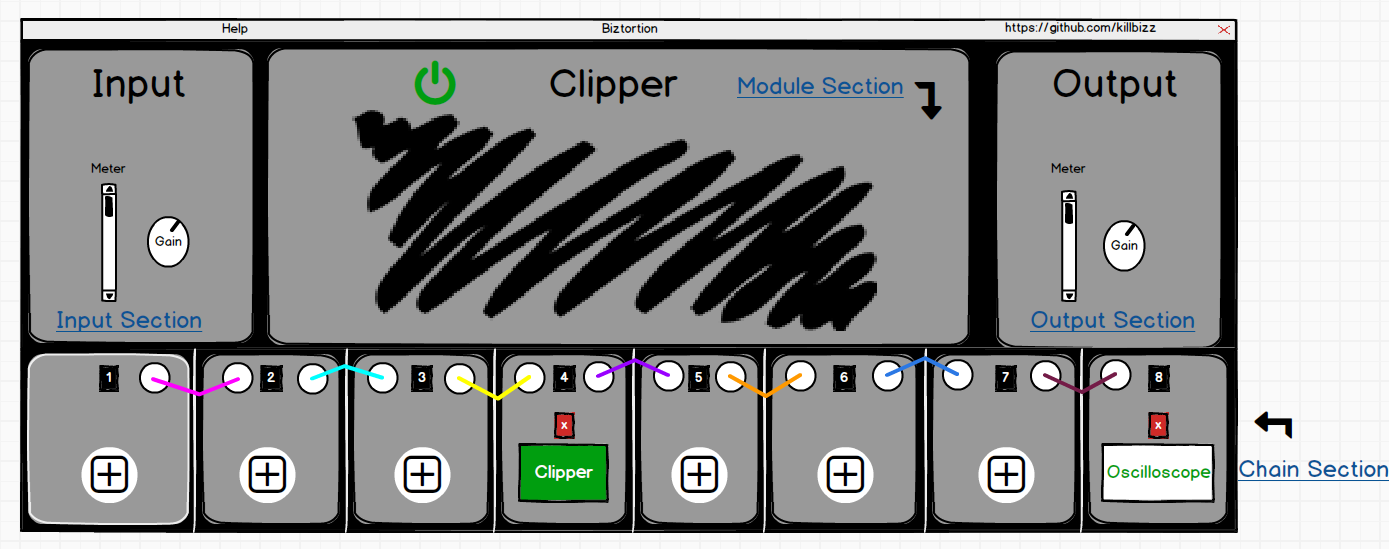
\includegraphics[width=0.9\columnwidth]{immagini/cap3/mockup1.png}
    \caption{Mockup della maschera principale del software Biztortion}
\end{figure}
Prima di procedere con la codifica del software è stata effettuata la progettazione della maschera principale, in modo da avere un'idea di base da cui partire e successivamente ampliare per la realizzazione dell'interfaccia grafica in base alle necessità. \\
Questo processo ha aiutato a definire in modo più accurato le componenti necessarie per il corretto funzionamento del software, identificando le componenti denominate \textit{Module Section}, \textit{Chain Section}, \textit{Chain Position}, \textit{Input Section} e \textit{Output Section}: le componenti in questione sono state quindi delineate e inserite nell'\hyperref[sez:analisi-requisiti]{analisi dei requisiti}. \\
Infine risulta utile notare che il \gls{mockupg} ottenuto, raffigurato nella figura 3.7, è stato realizzato con lo strumento \textit{Balsamiq Mockups}, descritto nella sezione 1.2.


\subsection{Architettura}
Il software in questione consiste in un \gls{pluging} audio realizzato utilizzando il framework \textbf{JUCE} sia per la parte logica di \gls{dspg} che per la parte di vista, ovvero la user interface. Il progetto di base, creato con lo strumento \gls{projucerg}, ha consentito lo sviluppo del software con un unico linguaggio di programmazione, ovvero il \textbf{C++}, grazie alla possibilità di creare diverse build nelle piattaforme Windows, MacOS e Linux. Nello specifico il software è stato esportato in formato \textbf{VST3} su \textbf{Windows} utilizzando lo strumento Microsoft Visual Studio, e in formato \textbf{AU} su \textbf{MacOS} attraverso lo strumento Xcode. \\ \\
I concetti fondamentali per l'implementazione di un \gls{pluging} audio utilizzando il framework JUCE sono le classi \textit{juce::AudioProcessor} e \textit{juce::AudioProcessorEditor}. Queste due classi corrispondono relativamente al processore di segnale audio (\gls{dspg}) e all'editor grafico (GUI) e, implementandole attraverso due classi concrete, rispettivamente \textit{BiztortionAudioProcessor} e \textit{BiztortionAudioProcessorEditor}, si ha la possibilità di definire i comportamenti del software una volta caricato nella \gls{dawg} desiderata. \\ \\
E' possibile notare nella figura 3.8 il \textbf{diagramma dei package} del software Biztortion, il quale permette di avere una chiara visione della struttura del progetto e delle strutture di supporto utilizzate all'interno delle classi \textit{BiztortionAudioProcessor} e \textit{BiztortionAudioProcessorEditor} per definire il comportamento del software.
\begin{figure}[h!] 
    \centering 
    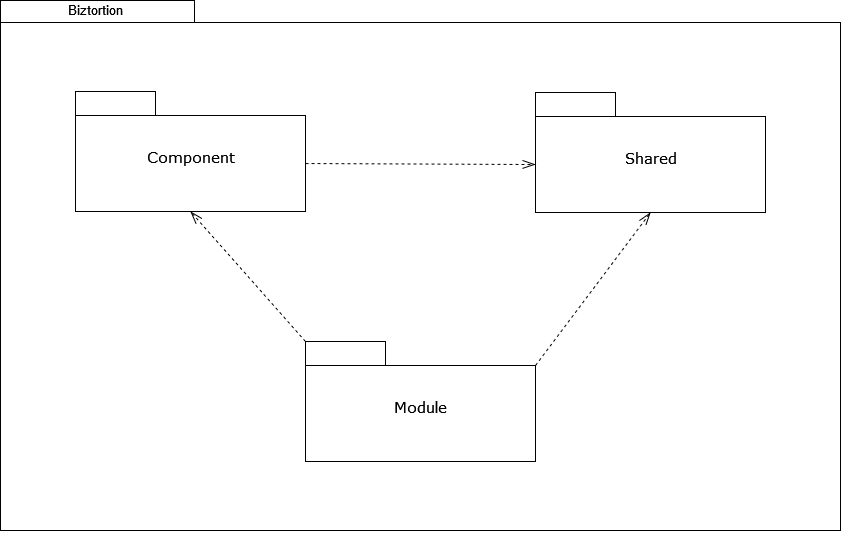
\includegraphics[width=0.9\columnwidth]{immagini/cap3/package.png}
    \caption{Diagramma dei package del software Biztortion}
\end{figure} \\
Gli elementi fondamentali dell'architettura sono i seguenti:
\begin{itemize}
    \item \textbf{Shared}: contiene tutte le strutture e classi di supporto utilizzate nei diversi moduli e component. Al suo interno sono presenti tutte le definizioni ed implementazioni dei componenti di utilità personalizzati per comporre la user interface (potenziometri e bottoni) oltre che ai componenti logici necessari per l'analisi della \gls{fftg};
    \item \textbf{Component}: contiene tutti i componenti grafici personalizzati, i quali  implementano la classe juce::Component e vengono utilizzati per illustrare informazioni in tempo reale all'interno di diversi moduli. In particolare sono presenti il FFTAnalyzerComponent, ResponseCurveComponent e TransferFunctionComponent;
    \item \textbf{Module}: contiene tutti i moduli istanziabili nella \textit{Chain Section}. Ogni modulo implementa due classi che permettono di standardizzare sia la parte di \gls{dspg} (\textit{DSPmodule}) sia la parte relativa all'interfaccia grafica (\textit{GUImodule}). Entrambe le classi, DSPmodule e GUImodule, vengono utilizzate rispettivamente da BiztortionAudioProcessor e BiztortionAudioProcessorEditor sfruttando il concetto di \gls{polimorfismog}, tipico della programmazione ad oggetti e disponibile col linguaggio di programmazione c++.
\end{itemize}

\subsection{Funzionalità implementate}
Il codice prodotto ha permesso di soddisfare la totalità dei requisiti, ovvero delle funzionalità necessarie evidenziate dai casi d'uso riscontrati durante l'\hyperref[sez:analisi-requisiti]{analisi dei requisiti}.
Con questo risultato si è arrivato ad avere un funzionamento completo del software \textit{Biztortion}, che verrà brevemente descritto in questa sezione.

\subsubsection*{Schermata principale}
La schermata principale del software è costituita dalle seguenti sezioni fondamentali, definite nel \hyperref[uc:1]{primo caso d'uso}:
\begin{itemize}
    \item \textbf{Module Section}: riservata alla visualizzazione dei moduli per l’audio processing o al pannello di benvenuto;
    \item \textbf{Chain Section}: riservata alla visualizzazione della catena di elaborazione del segnale, la quale può contenere moduli istanziati in un ordine arbitrario;
    \item \textbf{Input Section}: riservata al controllo del guadagno e il monitoraggio del segnale in ingresso;
    \item \textbf{Output Section}: riservata al controllo del guadagno e il monitoraggio del segnale in uscita;
\end{itemize}
\begin{figure}[h!] 
    \centering 
    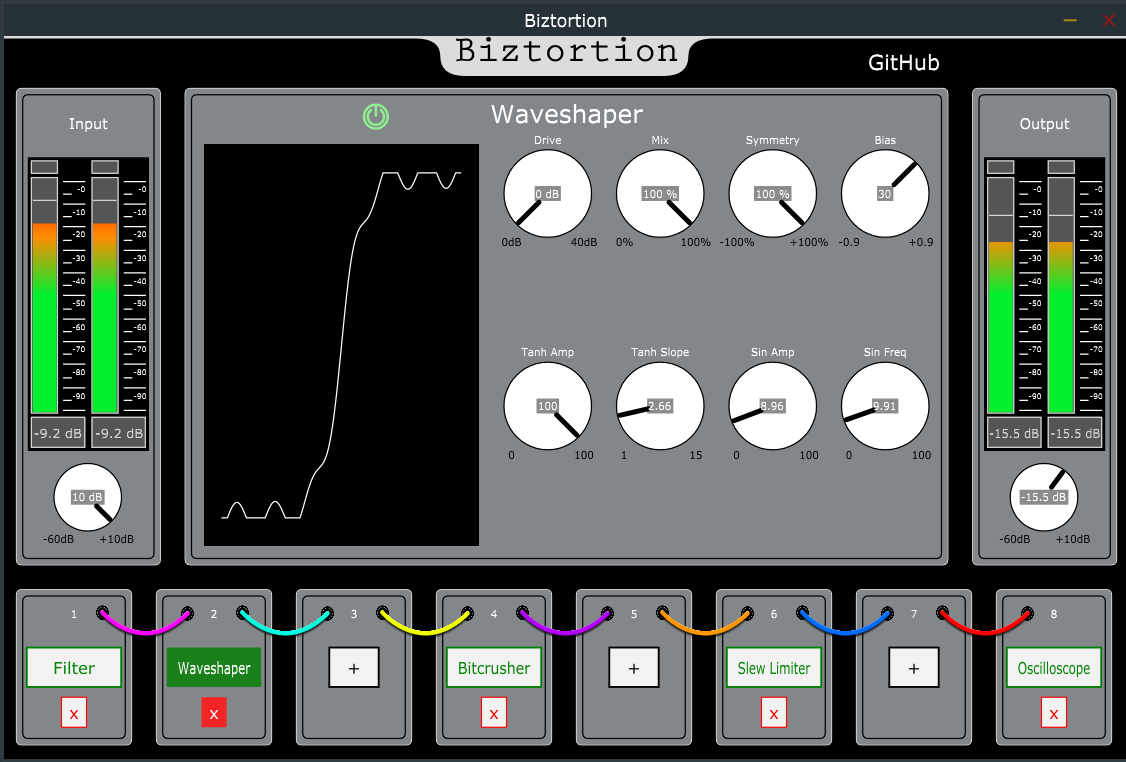
\includegraphics[width=0.9\columnwidth]{immagini/cap3/main.png}
    \caption{Biztortion: schermata principale e visualizzazione del modulo Waveshaper}
\end{figure}

\subsubsection*{Moduli}
Tutti i moduli presenti nel software (\textit{Oscilloscope}, \textit{Filter}, \textit{Waveshaper}, \textit{Bitcrusher}, \textit{Slew Limiter}) sono istanziabili dall'utente nella \textit{Chain Section} in un ordine arbitrario e implementano digitalmente le tecniche di distorsione del segnale analizzate nel \hyperref[cap:distorsione]{precedente capitolo}:
\begin{itemize}
    \item \textbf{Clipping}: è possibile effettuare il clipping del segnale in ingresso al \gls{pluging} utilizzando il modulo \textit{Waveshaper} per simulare l'effetto ottenibile con la strumentazione analogica. Grazie a questo modulo infatti risulta possibile utilizzare la funzione arcotangente con il potenziometro "tanh slope" al minimo e, regolando il potenziometro "drive", si può osservare un \textit{Soft Clipping}; per ottenere invece un \textit{Hard Clipping} è sufficiente aumentare in modo considerevole il potenziometro "drive" in quanto il modulo in questione, utilizzando anche la funzione seno che può causare l'uscita del segnale dai limiti -1/+1, ha un limitatore integrato che provvede a tagliare bruscamente il segnale nel caso superi il limite superiore o inferiore;
    \item \textbf{Waveshaping}: è possibile distorcere il segnale utilizzando la funzione di trasferimento composta presente nel modulo \textit{Waveshaper}, la quale utilizza le funzioni seno ed arcotangente, per creare varie forme d'onda molto complesse;
    \item \textbf{Bitcrushing}: è possibile ridurre la risoluzione del segnale utilizzando il modulo \textit{Bitcrusher} per intervenire sulla frequenza di campionamento e profondità di bit ed introdurre gradualmente gli artefatti digitali tipici dei vecchi campionatori;
    \item \textbf{Slew Limiting}: utilizzando il modulo \textit{Slew Limiter} è possibile impostare la soglia di velocità massima sopra alla quale essa stessa viene limitata nel tempo sul segnale in uscita, sia nella fase in cui l’onda si muove verso la zona positiva, sia durante la fase in cui l’onda procede nella direzione opposta, andando in questo modo a livellare il segnale in ingresso. \\
\end{itemize}
Inoltre tutti i moduli che effettuano la distorsione del segnale (\textit{Waveshaper}, \textit{Bitcrusher}, \textit{Slew Limiter}) possono applicare un algoritmo che gli consente di applicare l'effetto a tutta la forma d'onda o ad una sezione di essa, permettendo all'utente di decidere se e quanto effetto applicare in modo simmetrico o asimmetrico. \\ \\
L'utilizzo combinato dei moduli nella catena di elaborazione permette non solo di creare sonorità molto complesse, ma anche di ricreare effetti già collaudati e frequentemente utilizzati, come per esempio alcuni pedali per la distorsione del suono della chitarra elettrica attraverso le seguenti combinazioni:
\begin{itemize}
    \item \textbf{Overdrive}: utilizzando due moduli Filtro, posizionati prima e dopo un modulo Waveshaper, ed effettuando un'operazione di \gls{pre-enfasig} \textit{attenuando} le basse frequenze nel primo filtro è possibile ottenere un suono molto simile al tipico effetto overdrive;
    \item \textbf{Fuzz}: utilizzando due moduli Filtro, posizionati prima e dopo un modulo Waveshaper, ed effettuando un'operazione di \gls{pre-enfasig} \textit{enfatizzando} le basse frequenze nel primo è possibile ottenere un suono molto simile al tipico effetto fuzz.
\end{itemize}
Risulta utile infine citare che il software \textit{Biztortion} è stato testato manualmente su un sistema Windows 10 Home nelle seguenti \gls{dawg}:
\begin{itemize}
    \item Ableton Live Suite 11 (v. 11.0)
    \item Cycling'74 Max (v. 8.0.2 - 64 bit)
    \item Fruity Loops Studio (v. 12.1.2 - 64 bit)
    \item Reaper (v.6.38)
\end{itemize}